\chapter{Query Languages for Graph Databases}
\label{ch:prelim-graph-databases}

\begin{chapterpresentation}
	\begin{abstract}
		This preliminary chapter briefly surveys the literature on
		the notion of \emph{conjunctive queries},
		\emph{conjunctive regular path queries} and related notions.

		\todo{finish}
	\end{abstract}
	\par\bigskip\bigskip
	\begin{acknowledgements}
		Parts of this chapter come from the introduction and preliminaries of \cite{FigueiraMorvan2025SemanticTreeWidthLMCS,FigueiraMorvanRomero2025Minimizing}.
	\end{acknowledgements}
	\clearpagepresentation
	\chaptertocstandalone
\end{chapterpresentation}

In global prelims:
\begin{itemize}
	\itemAP $\intro*\surjto$
	\itemAP ""homomorphic image""
\end{itemize}

In prelims minimization:
\begin{itemize}
	\itemAP ""contracting edges""
	\itemAP ""minor"" and ""minor-closed""
\end{itemize}

\section{Relational Databases}

The most common model of databases is by far that of "relational databases",
in which data is stored in \emph{tables}: an example is depicted
in \Cref{fig:relational-database-cinema}.

\begin{table}
	\centering%
	{%
	\footnotesize%
	\begin{tabular}{cccc}
		\multicolumn{4}{c}{\textsc{Movies}} \\ \toprule
		id & title & length & director \\ \midrule
		197 & Eyes Wide Shut & 159 & Stanley Kubrick \\ 
		205 & J'ai tué ma mère & 96 & Xavier Dolan \\
		304 & Amadeus & 161 & Miloš Forman \\
		321 & 120 Battements par minute & 143 & Robin Campillo \\ \bottomrule
	\end{tabular}
	\\\bigskip%
	\begin{tabular}{cc}
		\multicolumn{2}{c}{\textsc{Rooms}} \\ \toprule
		id & capacity  \\ \midrule
		1 & 108 \\
		2 & 124 \\
		3 & 96 \\
		4 & 102 \\ \bottomrule
	\end{tabular}%
	\hspace{1cm}%
	\begin{tabular}{ccc}
		\multicolumn{3}{c}{\textsc{Projections}} \\ \toprule
		movie\_id & room\_id & time \\ \midrule
		197 & 2 & 2025-03-28 14:00 \\
		205 & 3 & 2025-03-28 14:30 \\
		321 & 4 & 2025-03-28 14:30 \\
		197 & 1 & 2025-03-28 17:00 \\ \bottomrule
	\end{tabular}
}
	\caption{
		\AP\label{fig:relational-database-cinema}
		A "relational database" consisting of three tables, representing data
		stored by a cinema. (Replica of \Cref{fig:example-db-as-rel}.)
	}
\end{table}

\todo{we will not mention relational algebra, see \cite[\S\!\S~2--7]{ArenasBarceloLibkinMartensPieris2022DatabaseTheory}.}

\begin{itemize}
	\item duality w/ table of equivalence (vertex <-> variable ; disjoint union <-> disjoint conjunctions)
	\itemAP $\intro*\underlying{\gamma}$ and ""underlying graph""
	\itemAP ""relational database""
	\itemAP ""equality atom""
	\itemAP ""evaluation map@@cq"" (explain why notion is necessary by pointing to "evaluation map" for CRPQs)
	\itemAP ""disjunct""
	\itemAP ""conjunctive query evaluation""
\end{itemize}

\section{Intermezzo: Parametrized Complexity Classes}

\begin{itemize}
	\itemAP ""FPT""
	\itemAP ""W1""
	\itemAP ""XP""
\end{itemize}

\section{Graph Databases}

\begin{itemize}
	\itemAP $\intro*\Exp$ and ""expansion""
	\itemAP $\intro*\cdb$ and ""canonical database""
	\itemAP $\intro*\Refin$, ""atom refinement"", ""refinement""
	\itemAP $\intro*\contract{L_i \cdots L_{j}}$, ""one-way contraction"", ""contraction"" and ""condensation"" -> unify terminology; ""contracting internal variables"", ""internal path""
	\itemAP $\intro*\nbatoms{\gamma}$, $\intro*\nbvar{\gamma}$
	\itemAP ""evaluation map""
	\itemAP ""simple regular expression"" and ""positive simple regular expression""
\end{itemize}

A \AP""class of (Boolean) CRPQs"" is a function \AP$\intro*\classCRPQ$ mapping an alphabet $\A$ 
to a set $\classCRPQ_{\A}$ of "Boolean CRPQs", which is closed under variable renaming and alphabetic
renaming of the languages.

% % ---
% % Minimization paper
% % ---

% \paragraph{Graph databases.}
% \AP ""Graph databases"" are abstracted as edge-labelled directed graphs
% $G = \langle \vertex{G}, \edges{G} \rangle$, 
% where nodes of $\intro*\vertex{G}$ represent entities and labelled edges $\intro*\edges{G} \subseteq \vertex G \times \A \times \vertex G$
% represent relations between these entities, with $\A$ being a fixed finite alphabet.

% \paragraph{Conjunctive regular path queries (CRPQs) and unions of CRPQs (UCRPQs).}
% \AP A ""CRPQ"" $\gamma$ is defined as a tuple $\bar z = (z_1,\hdots,z_n)$
% of ""output variables""\footnote{For technical reasons (see the definition of "equality atoms") we allow for a variable to appear multiple times.},
% together with a conjunction of ""atoms"" of the form
% \AP$\bigwedge_{j=1}^m x_j \intro*\atom{L_j} y_j$, where each $L_j$ is a regular language
% and where $m \geq 0$.
% The set of all variables occurring in $\gamma$, namely%
% \footnote{We neither assume 
% disjointness nor inclusion between $\{z_1,\hdots,z_n\}$ and $\{x_1,y_1,\hdots,x_m,y_m\}$.}
% $\{z_1,\hdots,z_n\}\cup\{x_1,y_1,\hdots,x_m,y_m\}$, is denoted by
% $\intro*\vars(\gamma)$. Variables in $\vars(\gamma)\setminus \{z_1,\hdots,z_n\}$ are existentially quantified. 
% We denote by $\intro*\atoms(\gamma)$ the set of "atoms" of $\gamma$.
% Given a "database@@graph" $G$, we say that a tuple of nodes $\bar u = (u_1,\hdots,u_n)$
% \AP""satisfies@@db"" $\gamma$ 
% on $G$ if there is a mapping
% $\fun\colon \vars(\gamma) \to \vertex{G}$ such that $u_i = \fun(z_i)$ for all
% $1 \leq i \leq n$, and for each $1 \leq j \leq m$,
% there exists a (directed) path from $\fun(x_j)$ to $\fun(y_j)$ in $G$, labelled by
% a word from $L_j$ (if the path is empty, the label is $\varepsilon$). The \AP""evaluation"" of $\gamma$ on $G$ is then the set of all tuples that "satisfy@@db" $\gamma$ on $G$.

% A ""union of CRPQs"" (\reintro{UCRPQs})
% is defined as a finite set of "CRPQs", called \AP""disjuncts"", whose tuples of "output variables" have all the same arity.
% The "evaluation" of a union is defined as the union of its "evaluations". 
% If a query has no "output variables" we call it ""Boolean"", and
% its "evaluation" can either be the set $\set{()}$, in which case we say that $G$
% \reintro(db){satisfies} the query, or the empty set $\set{}$.

% \AP Given two "UCRPQs" $\Gamma$
% and $\Gamma'$ whose "output variables" have the same arity,
% we say that $\Gamma$ is \AP""contained"" in $\Gamma'$,
% denoted by $\Gamma \intro*\contained \Gamma'$, if
% for every "graph database" $G$, for every tuple $\bar u$ of $\vertex{G}$,
% if $\bar u$ "satisfies@@db" $\Gamma$ on $G$, then so does $\Gamma'$. We will hence reserve the symbol `$\subseteq$' for set inclusion.
% The \AP""containment problem"" for "UCRPQs" is the problem of, given
% two "UCRPQs" $\Gamma$ and $\Gamma'$, to decide if $\Gamma \contained \Gamma'$.
% When $\Gamma \contained \Gamma'$ and $\Gamma' \contained \Gamma$  we say that
% $\Gamma$ and $\Gamma'$ are \AP""equivalent"", denoted by
% $\Gamma \intro*\semequiv \Gamma'$. 

% \AP A ""conjunctive query"" (\reintro{CQ}) is in this context a "CRPQ" whose every atom is of the form $x \atom{a} y$ for $a \in \A$ ("ie", every language is a singleton $\set{a}$).
% \AP A ""union of CQs"" (\reintro{UCQs}) is defined as a "UCRPQ" with the same property.

% A \AP""canonical database"" $G$ of a "CRPQ" $\gamma$ is any "canonical database" associated
% to an "expansion" of $\gamma$, see \cite[Definition 3.1]{FlorescuLevySuciu1998Containment}
% for a formal definition. We denote it by \AP$G \intro*\cdb \gamma$.
% A \reintro{canonical database} of a "UCRPQ" is a "canonical database" of one
% of its "disjuncts".

% An \AP""evaluation map"" from a "CRPQ" $\gamma$ to a "graph database" $G$
% in a function $f$ from variables of $\gamma$ to $G$ "st"
% for any atom $x \atom{L} y$ in $\gamma$, there is path from $f(x)$ to $f(y)$ in $G$
% labelled by a word of $L$.

% The "containment" between "UCRPQs" $\Gamma_1 \contained \Gamma_2$ is exactly characterized
% by the fact that for all "canonical database" $G_1 \cdb \Gamma_1$,
% there exists a "disjunct" $\gamma_2$ of $\Gamma_2$ "st" there is an "evaluation map"
% from $\gamma_2$ to $G_1$.

% \paragraph{Homomorphisms.}
% \AP A ""homomorphism"" $\fun$ from a "CRPQ" $\gamma(x_1, \dotsc, x_m)$ to a "CRPQ" $\gamma'(y_1, \dotsc, y_m)$ is a mapping from $\vars(\gamma)$ to $\vars(\gamma')$ such that $\fun(x) \atom{L} \fun(y)$ is an "atom" of $\gamma'$ for every "atom" $x \atom{L} y$ of $\gamma$, and further $\fun(x_i)=y_i$ for every $i$.
% Such a "homomorphism" $\fun$ is \AP""strong onto"" if for every "atom" $x' \atom{L} y'$ of $\gamma'$ there is an "atom" $x \atom{L} y$ of $\gamma$ such that $\fun(x)=x'$ and $\fun(y)=y'$.
% % An example of "homomorphism" is provided in \Cref{fig:basic-hom}.
% We write $\gamma \intro*\homto \gamma'$ if there is a "homomorphism" from $\gamma$ to $\gamma'$, and $\gamma \intro*\surjto \gamma'$ if there is a "strong onto homomorphism".
% In the latter case, we say that $\gamma'$ is a \AP""homomorphic image"" of $\gamma$.
% A \reintro{homomorphism} $\fun$ from a graph database $G$ to a graph database $G'$ is a mapping from $\vertex{G}$ to $\vertex{G'}$ such that  for every edge $u \atom{a} v$ of $G$, it holds that $\fun(u) \atom{a} \fun(v)$ is an edge in $G'$. A "homomorphism" from a "CQ" to a graph database is defined analogously.  

% \AP It is easy to see that if $\gamma \homto \delta$ then $\delta \contained \gamma$, and in the case where $\gamma,\delta$ are "CQs" this is an ``if and only if'' \cite[Lemma 13]{ChandraMerlin1977Implementation}. 
% \AP Two "CQs" $\gamma,\delta$ are ""hom-equivalent"" if there are "homomorphisms" $\gamma \homto \delta$ and $\delta \homto \gamma$.
% Hence, for any two "CQs" $\gamma, \delta$, we have $\gamma \semequiv \delta$ if, and only if, they are "hom-equivalent".
% \AP The ""core"" of a "CQ" $\gamma$, denoted by $\intro*\core(\gamma)$
% is the result of repeatedly removing any atom which results in an equivalent query. It is unique up to isomorphism (see, "eg", \cite{ChandraMerlin1977Implementation}). We say that a "CQ" is `a core' if it is isomorphic to its "core". If $\gamma$ and $\delta$ are "hom-equivalent" then they have
% the same "core". Moreover, there is always an \AP""embedding""---"ie", a "homomorphism" which is injective both on variables and "atoms"---of $\core(\gamma)$ into $\gamma$.

% \paragraph*{Refinements and expansions of (U)CRPQs.}
% \AP For an NFA $\+A$ and two states $q,q'$ thereof, we denote by $\intro*\subaut{\+A}{q}{q'}$ the ""sublanguage"" of $\+A$ recognized  when considering $\set{q}$ as the set of initial states and $\set{q'}$ as the set of final states.
% \AP An ""atom $m$-refinement"" of a "CRPQ" "atom" $\gamma(x,y) = x \atom{L} y$ where $m\geq 1$ and $L$ is given by the NFA $\+A_L$ is any "CRPQ" of the form 
% \begin{equation}
% 	\AP\label{eq:refinement}
% 	\rho(x,y) = x \atom{L_1} t_1 \atom{L_2} \hdots \atom{L_{n-1}} t_{n-1} \atom{L_n} y
% \end{equation}
% where $1 \leq n \leq m$, $t_1,\hdots,t_{n-1}$ are fresh (existentially quantified) variables,
% and $L_1,\hdots,L_n$ are such that there exists a sequence $(q_0,\dotsc,q_n)$ of states of $\+A_L$
% such that $q_0$ is initial, $q_n$ is final, and for each $i$, $L_i$ is either of the form
% \begin{enumerate}[label=\roman*.]
% 	\item $\subaut{\+A_L}{q_{i-1}}{q_{i}}$, or 
% 	\item $\{a\}$ if the letter $a\in \A$ belongs to $\subaut{\+A_L}{q_{i-1}}{q_{i}}$.
% \end{enumerate}
% Additionally, if $\varepsilon \in L$, the \AP""equality atom"" ``$x = y$'' is also an \reintro{atom $m$-refinement}. Thus, an \reintro{atom $m$-refinement} can be either of the form \eqref{eq:refinement} or ``$x=y$''.
% By definition, note that the concatenation
% $L_1\cdots L_n$ is a subset of  $L$ and hence $\rho \contained \gamma$ for any "atom $m$-refinement" $\rho$ of $\gamma$.
% An \AP""atom refinement"" is an "atom $m$-refinement" for some $m$.

% Given a natural number $m$, an \AP""$m$-refinement"" of a "CRPQ" $\gamma(\bar x) = \bigwedge_{i} x_i \atom{L_i} y_i$ is any query resulting from: (1) replacing every "atom" by one of its "$m$-refinements@@atom", and (2)
% should some "$m$-refinements@@atom" have "equality atoms",
% collapsing the variables (and removing the identity atoms `$x=x$').
% \AP A ""refinement"" is an "$m$-refinement" for some $m$.
% Note that in a "refinement" of a "CRPQ"
% the "atom refinements" need not have the same length.
% For instance, both $\rho(x,x) = x \atom{c} x$ and $\rho'(x,y) = x \atom{a} t_1 \atom{a} y \coatom{c} y$ are "refinements" of $\gamma(x,y) = x \atom{a^*} y \coatom{c} x$.
% \AP
% We write $\intro*\Refin(\gamma(\bar x))$ to denote the set of all "refinements" of $\gamma(\bar x)$ and $\reintro*\Refin[\leq m](\gamma(\bar x))$ to the $m$-refinements. 

% The set of \AP""expansions"" of a "CRPQ" $\gamma$ is the set $\intro*\Exp(\gamma)$ of all "CQs" which are "refinements" of $\gamma$.
% In other words, an "expansion" of $\gamma$ is any "CQ" obtained from $\gamma$
% by replacing each "atom" $x \atom{L} y$ by a path $x \atom{w} y$ for some
% word $w \in L$. The "expansions" (resp.\ "refinements") of a "UCRPQ" are the "expansions" (resp.\ "refinements") of the "CRPQs" it contains.
% We define \AP""atom expansions"" analogously to "atom refinements". For "UCRPQs" we use  $\Exp(\Gamma)$, $\Refin(\Gamma)$ and $\Refin[\leq m](\Gamma)$ as for "CRPQs".

% Any "UCRPQ" is equivalent to the infinitary union of its "expansions". In light of this, 
% the semantics for "UCRPQs" can be rephrased as follows. 
% Given a "UCRPQ" $\Gamma(\bar x)$ and a graph database $G$, 
% the "evaluation" of $\Gamma(\bar x)$ on $G$, denoted by $\Gamma(G)$, is the set of tuples 
% $\bar{v}$ of nodes for which there is $\anexpansion \in \Exp(\Gamma)$ such that there is a "homomorphism" $\anexpansion \homto G$ that sends $\bar x$ onto $\bar v$. 

% "Containment" of "UCRPQs" can also be characterized in terms of "expansions".
% \begin{proposition}[Folklore, see e.g. {\cite[Proposition 3.2]{FlorescuLevySuciu1998Containment}} or
% 	{\cite[Theorem 2]{CalvaneseDeGiacomoLenzeriniVardi2000Containment}}]
% 	\AP\label{prop:cont-char-exp-st} 
% 	Let $\Gamma_1$ and $\Gamma_2$ be "UCRPQs". Then the following are equivalent:
% 	% \begin{itemize}
% 		% \item 
% 		(i) $\Gamma_1 \contained \Gamma_2$;
% 		% \item 
% 		(ii) for every $\anexpansion_1\in \Exp(\Gamma_1)$, $\anexpansion_1 \contained \Gamma_2$;
% 		% \item 
% 		(iii) for every $\anexpansion_1\in \Exp(\Gamma_1)$ there is $\anexpansion_2\in \Exp(\Gamma_2)$ such that $\anexpansion_2\homto \anexpansion_1$. 
% 	% \end{itemize}
% \end{proposition}

% \begin{hypothesis}
% 	To simplify proofs, we often assume that the regular languages are described via non-deterministic finite automata (NFA) instead of regular expressions,
% 	which does not affect any of our complexity bounds.
% 	However, for readability all our examples will be given in terms of regular expressions.
% \end{hypothesis}

% \AP We denote by $\intro*\nbatoms{\gamma}$ the number of "atoms" of a "CRPQ" $\gamma$ and by $\intro*\nbvar{\gamma}$ the number of variables.
% We extend these notations to a "UCRPQ" $\Gamma$ by letting
% $\nbatoms{\Gamma} = \max_{\gamma \in \Gamma} \nbatoms{\gamma}$
% and $\nbvar{\Gamma} = \max_{\gamma \in \Gamma} \nbvar{\gamma}$. 
% We denote by $\size{\Gamma}$ the size (of a reasonable encoding) of a  "UCRPQ". 
% For a CRPQ $\gamma$, we define its  \AP""underlying graph"" $\intro*\underlying{\gamma}$ of $\gamma$ as the directed multigraph obtained from $\gamma$ by ignoring the regular languages labelling the atoms of $\gamma$. 

% We assume familiarity with basic concepts of directed multigraphs.
% For simplicity, thorough the paper, by `graph' we mean a directed multigraph. We also adapt implicitly in the natural way, concepts defined for "CRPQs" to (directed multi)graphs (such a "homomorphisms", "embeddings", etc.).
% A \AP""minor"" of a graph is any graph that can be obtained by removing
% edges, removing vertices---and their adjacent edges---, and \AP""contracting edges""---meaning that we identify the two endpoints of the edge and remove the edge from the graph.%
% \footnote{This definition is a trivial generalization of the notion of minors for undirected graphs.}

% Formally, a \AP""contraction@@var"" of an "internal variable" $y$ in a "CRPQ" $\gamma$ is the result of replacing any pair of distinct atoms $x \atom{L} y$ and $y \atom{L'} z$ with $x \atom{L \cdot L'} z$ for $L \cdot L' \defeq \set{w \cdot w' : w \in L, w' \in L'}$.%
% \footnote{Note that "contraction of internal variable" is a particular case of "edge contraction".} Observe that this results in an "equivalent" query.
% A \AP""contraction"" of $\gamma$ is any "CRPQ" obtained by repeatedly "contracting@@var" "internal variables".

% % ---
% % Semantic tree-width
% % ---

% Before attacking the statement of our "Key Lemma" in \Cref{sec:maximal-under-approximations},
% we first give a few elementary definitions on "C2RPQs" in this section.
% %
% % \paragraph*{Homomorphisms}
% \AP
% A homomorphism $\fun$ from a "C2RPQ" $\gamma(x_1, \dotsc, x_m)$ to a "C2RPQ" $\gamma'(y_1, \dotsc, y_m)$ is a mapping from $\vars(\gamma)$ to $\vars(\gamma')$ such that $\fun(x) \atom{L} \fun(y)$ is an "atom" of $\gamma'$ for every "atom" $x \atom{L} y$ of $\gamma$, and further $\fun(x_i)=y_i$ for every $i$.
% Such a "homomorphism" $\fun$ is \AP""strong onto"" if for every "atom" $x' \atom{L} y'$ of $\gamma'$ there is an "atom" $x \atom{L} y$ of $\gamma$ such that $\fun(x)=x'$ and $\fun(y)=y'$.
% An example of "homomorphism" is provided in \Cref{fig:basic-hom}.
% We write $\gamma \homto \gamma'$ if there is a "homomorphism" from $\gamma$ to $\gamma'$, and $\gamma \surj \gamma'$ if there is a "strong onto homomorphism".
% \todo{change this shit}
% In the latter case, we say that $\gamma'$ is a \AP""homomorphic image"" of $\gamma$.
% It is easy to see that if $\gamma \homto \gamma'$ then $\gamma' \contained \gamma$, and in the case where $\gamma,\gamma'$ are "CQs" this is an ``if and only if'' \cite[Lemma~13]{ChandraMerlin1977Implementation}.

% \paragraph*{Some intuitions on maximal under-approximations}
% Given a "conjunctive query" $\gamma$,
% the union of all "conjunctive queries"
% that are "contained" in $\gamma$ is "semantically equivalent" to the union
% $\bigvee \{ \gamma' \mid \gamma \surj \gamma' \}$. Naturally, this statement borders on the trivial since $\gamma'$ belongs to this union. It becomes interesting when we add a restriction:
% given a class $\class$ of "CQs" (to which $\gamma$ may not belong) closed under "subqueries", then $\Gamma' \defeq \bigvee \{ \gamma' \in \class \mid \gamma \surj \gamma' \}$ is the maximal under-approximations
% of $\gamma$ by finite unions of "conjunctive queries" of $\class$, in the following sense:
% \begin{enumerate}[label=\roman*.]
% 	\item (finite) $\Gamma'$ is a finite union of "CQs" of $\class$,
% 	\item (under-approximation) $\Gamma' \contained \gamma$, and
% 	\item (maximality) for any finite union $\Delta$ of "CQs" of $\class$, if $\Delta \contained \gamma$, then $\Delta \contained \Gamma'$.
% \end{enumerate}

% \begin{proof}
% Only the last point is non-trivial, and follows from the fact that if
% $\Delta \contained \gamma$, then for each $\delta \in \Delta$, $\delta \contained \gamma$,
% so there is a "homomorphism" $f\colon \gamma \to \delta$. The image $\delta'$
% of $f$ is a "subquery" of $\delta$, and $\+C$ is closed under "subqueries",
% so it belongs to $\+C$, and hence to $\Gamma'$. Since there is a trivial homomorphism
% from $\delta'$ to $\delta$, we moreover have that $\delta \contained \delta'$.
% Hence, for each "CQ" $\delta \in \Delta$, there is a CQ $\delta' \in \Gamma'$ such
% that $\delta \contained \delta'$, and hence $\Delta \contained \Gamma'$.
% \end{proof}

% As a consequence, we deduce that for each $k \geq 1$,
% the "maximal under-approximation" of a "CQ" by
% a finite union of "CQs" of "tree-width" at most $k$ is computable, and hence
% we can effectively decide if some "CQ" is "equivalent" to a query of "tree-width" at
% most $k$ by testing the equivalence with this maximal under-approximation.
% For more details on approximations of "CQs", see \cite{BarceloLibkinRomero2014Efficient}.
% Note that interestingly, changing $\Gamma'$ from
% $\bigvee \{ \gamma' \in \class \mid \gamma \surj \gamma' \}$
% to $\bigvee \{ \gamma' \in \class \mid \gamma' \contained \gamma \}$
% preserves both under-approximation and maximality, but $\Gamma'$ is now an infinite
% union of "CQs" of $\+C$.

% Unfortunately, these results cannot be straightforwardly extended to "conjunctive regular
% path queries" since the previous proof implicitly relied on two points:
% \begin{enumerate}
% 	\item the equivalence between the
% 	"containment" $\gamma' \contained \gamma$ and the existence of a "homomorphism"
% 	$\gamma \homto \gamma'$, and
% 	\item the possibility to restrict $\gamma'$ to its image $\gamma \homto \gamma'$ while 
% 	obtaining a semantically bigger query.
% \end{enumerate}
% These two crucial ingredients is what allows us to build a finite set $\Gamma'$ from $\gamma$.
% For "CRPQs", the second point still holds, but not the first one.
% For instance, the "CQ" $\gamma(x,y) = x \atom{a} z \atom{b} y$ is
% contained in (in fact "equivalent" to) the "CRPQ" $\gamma'(x,y) = x \atom{ab} y$,
% but there is no "homomorphism" from $\gamma'(x,y)$ to $\gamma(x,y)$.
% Our main result shows that to find "maximal under-approximations" of "C2RPQs",
% it suffices to take "homomorphic images" of so-called ``"refinements"'' of $\gamma$,
% instead of "homomorphic images" of $\gamma$ itself. The next paragraphs are devoted to
% introducing "refinements" and tools related to them.

% \paragraph*{Equality Atoms}
% \AP"C2RPQs" with ""equality atoms"" are queries of the form $\gamma(\bar{x}) = \delta \land I$, 
% where $\delta$ is a "C2RPQ" (without equality atoms) and $I$ is a conjunction of "equality atoms" of the form $x=y$. 
% Again, we denote by $\vars(\gamma)$ the set of variables appearing in the (equality and non-equality) atoms of $\gamma$. 
% We define the binary relation $=_\gamma$ over $\vars(\gamma)$ to be the reflexive-symmetric-transitive closure of the binary relation $\{(x, y) \mid \text{$x=y$ is an "equality atom" in $\gamma$}\}$. 
% In other words, we have $x=_\gamma y$ if the equality $x=y$ is forced by the "equality atoms" of $\gamma$. 
% Note that every "C2RPQ" with "equality atoms" $\gamma(\bar{x}) = \delta \land I$ is equivalent to a "C2RPQ" without "equality atoms"  $\gamma^{\collapse}$, 
% which is obtained from $\gamma$ by collapsing each equivalence class of the relation $=_\gamma$ into a single variable. 
% This transformation gives us a \emph{canonical} renaming from $\vars(\gamma)$ to $\vars(\gamma^{\collapse})$. For instance, $\gamma(x,y) \defeq x \atom{K} y \land y \atom{L} z \land x = y$
% collapses to $\gamma^{\collapse}(x,x) \defeq x \atom{K} x \land x \atom{L} z$.

% \paragraph*{Refinements}
% \AP An ""atom $m$-refinement"" of a "C2RPQ" "atom" $\gamma(x,y) = x \atom{L} y$ where $L$ is given by the NFA $\+A_L$ is any "C2RPQ" of the form 
% \begin{equation}
%     \AP\label{eq:refinement}
%     \rho(x,y) = x \atom{L_1} t_1 \atom{L_2} \hdots \atom{L_{n-1}} t_{n-1} \atom{L_n} y
% \end{equation}
% where $1 \leq n \leq m$, $t_1,\hdots,t_{n-1}$ are fresh (existentially quantified) variables,
% and $L_1,\hdots,L_n$ are such that there exists a sequence $(q_0,\dotsc,q_n)$ of states of $\+A_L$
% such that $q_0$ is initial, $q_n$ is final, and for each $i$, $L_i$ is either of the form
% \begin{enumerate}[label=\roman*.]
% 	\item $\subaut{\+A_L}{q_i}{q_{i+1}}$,
% 	\item $\{a\}$ if the letter $a\in \A$ belongs to $\subaut{\+A_L}{q_i}{q_{i+1}}$, or 
% 	\item $\{a^{-}\}$ if $a^{-} \in \A^{-}$ belongs to $\subaut{\+A}{q_i}{q_{i+1}}$.
% \end{enumerate}
% Additionally, if $\epsilon \in L$, the "equality atom" ``$x = y$'' is also an \reintro{atom $m$-refinement}. Thus, an \reintro{atom $m$-refinement} can be either of the form \eqref{eq:refinement} or ``$x=y$''.
% By convention, $t \atom{a^{-}} t'$ is a shorthand for $t' \atom{a} t$. As a consequence,
% the underlying graph of an "atom $m$-refinement" of the form \eqref{eq:refinement} is not necessarily a directed path.
% By definition, note that
% $L_1\cdots L_n \subseteq L$ and hence $\rho \contained \gamma$ for any "atom $m$-refinement" $\rho$ of $\gamma$.
% An \AP""atom refinement"" is an "atom $m$-refinement" for some $m$.
% An example is provided in \Cref{fig:basic-refinement}.

% \begin{marginfigure}
% 	\centering
% 	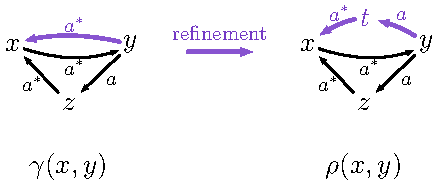
\includegraphics[width=\linewidth]{basic-refinement.pdf}
% 	\caption{\AP\label{fig:basic-refinement}A "refinement".}
% \end{marginfigure}
	
% \begin{marginfigure}
% 	\centering
% 	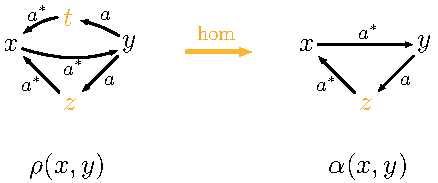
\includegraphics[width=\linewidth]{basic-hom.pdf}
% 	\caption{\AP\label{fig:basic-hom}A "strong onto homomorphism".}
% \end{marginfigure}

% \begin{definition}
%     \AP\label{def:atom-contraction}
%     \AP Given an "atom refinement" $\rho = x \atom{L_1} t_1 \atom{L_2} \hdots \atom{L_{n-1}} t_{n-1} \atom{L_n} y$ of $\gamma = x \atom{L} y$ as in \eqref{eq:refinement}, define
%     a ""condensation"" of $\rho$ between $t_i$ and $t_j$, where $0 \leq i,j \leq n$ and $j > i+1$, as any "C2RPQ" of the form:
%     \[
%         \rho' = x \atom{L_1} t_1 \atom{L_2} \hdots \atom{L_i} \textcolor{cPurple}{t_i \atom{K} t_j} \atom{L_{j+1}} \hdots
%         \atom{L_{n-1}} t_{n-1} \atom{L_n} y
%     \]
%     such that $\textcolor{cPurple}{K = \+A[q_i,q_j]}$.
% 	\begin{fact}
% 		\AP\label{fact:refinement-contained}
% 		Every "condensation" $\rho'$ of $\rho$ is a "refinement" of $\gamma$, and $\rho \contained \rho' \contained \gamma$.
% 	\end{fact}
%     \AP Informally, we will abuse the notation and
%     write $\intro*\contract{L_{i}\cdots L_{j}}$ to denote the language $K$---even if this language
%     does not only depend on $L_{i}\cdots L_{j}$.
% \end{definition}

% \begin{example}
%     \AP\label{ex:atom-refinement-twoway}
%     Let $\gamma(x,y) = x \atom{(aa^-)^*} y$ be a "C2RPQ" "atom", where
%     $(aa^-)^*$ is implicitly represented by its minimal automaton.
%     Then $\rho(x,y)$ is a "refinement" of "refinement length" seven of $\gamma(x,y)$
%     and $\rho'(x,y)$ is a "condensation" of $\rho(x,y)$, where:
%     \begin{align*}
%         \rho(x,y) & = x \atom{a} t_1 \atom{(a^-a)^*} t_2 \atom{(a^-a)^*} t_3
%             \coatom{a} t_4 \atom{(aa^-)^*} t_5 \atom{(aa^-)^*a} t_6 \coatom{a} y, \\
%         \rho'(x,y) & = x \atom{a} t_1 \atom{(a^-a)^*} t_2 \atom{(a^-a)^*} t_3
% 		\coatom{a} t_4 \atom{(aa^-)^*} y. 
%     \end{align*}
%     On the other hand, $\rho''(x,y) = x \atom{a} t_1 \coatom{a} y$ is not
%     a "condensation" of $\rho(x,y)$.
% \end{example}

% Given a natural number $m$, an \AP""$m$-refinement"" of a "C2RPQ" $\gamma(\bar x) = \bigwedge_{i} x_i \atom{L_i} y_i$ is any query resulting from: 1) replacing every "atom" by one of its "$m$-refinements@@atom", and 2)
% should some "$m$-refinements@@atom" have "equality atoms",
% collapsing the variables.
% \AP A ""refinement"" is an "$m$-refinement" for some $m$.
% Note that any "atom $m$-refinements" is, by definition, also an
% "atom $m'$-refinements" when $m \leq m'$: as a consequence, in the "refinement" of a "C2RPQ"
% the "atom refinements" need not have the same length.
% For instance, both $\rho(x,x) = x \atom{c} x$ and $\rho'(x,y) = x \atom{a} t_1 \atom{a} y \coatom{c} y$ are "refinements" of $\gamma(x,y) = x \atom{a^*} y \coatom{c} x$.

% %%%%%%%%%%%%%%%%%%%%%
% %     We will assume that a query "refinement" does not contain atoms with the language $\set{\epsilon}$; these are eliminated by identifying variables in a standard way. For example, if the result of replacing atoms by "atom refinements" yields $\gamma(x,z) = x \atom{\set{\epsilon}} y \land y \atom{\set{\epsilon}} z \land z \atom{a^*} x$ the associated "refinement" is then $\gamma(x,x) =  x \atom{a^*} x$.
% % \sidediego{CHECK}
% %%%%%%%%%%%%%%%%%%%%%
% For a given "C2RPQ" $\gamma$, let $\AP\intro*\Refin[\leq m](\gamma)$ be the set of all "$m$-refinements" of $\gamma$, and $\reintro*\Refin(\gamma)$ be the set of all its "refinements".
% Given a "refinement" $\rho(\bar x)$ of $\gamma(\bar x)$,
% its ""refinement length"" is the least natural number
% $m$ such that $\rho(\bar x) \in \Refin[\leq m](\gamma)$.
% Note that if the automaton representing a language $L$ has more than one final state, for instance the minimal automaton for $L = a^+ + b^+$,
% then $x \atom{L} y$ is not a "refinement" of itself.
% However, it will always be "equivalent" to a union of refinements: in
% this example, $x \atom{a^+ + b^+} y$ is "equivalent" to the union of
% $x \atom{a^+} y$ and $x \atom{b^+} y$, which are both "refinements"
% of the original "C2RPQ".

% \paragraph*{Expansions}
% %%%%%%%%%%%%%%%%%%%%%
% % \sidediego{CHECK}
% % Observe that a "C2RPQ" $\gamma$ whose every language is of the form $\set{z}$ for $z \in \Aext \dcup \set{\varepsilon}$ is equivalent to a "conjunctive query" $\tilde \gamma$. For example, $\gamma(x,y) = x \atom{\varepsilon} y \land y \atom{\set{a^-}} z$ is equivalent to $\tilde\gamma(y,y) = z \atom{a} y$. 
% Remember that a "C2RPQ" whose languages are
% of the form $\set{a}$ or $\set{a^-}$ for $a \in \A$ is in effect a "CQ".
% The \AP""expansions"" of a "C2RPQ" $\gamma$ is the set $\intro*\Exp(\gamma)$ of all "CQs" which are "refinements" of $\gamma$.
% In other words, an "expansion" of $\gamma$ is any "CQ" obtained from $\gamma$
% by replacing each "atom" $x \atom{L} y$ by a path $x \atom{w} y$ for some
% word $w \in L$.
% For instance, $\xi(x,y) = x \atom{a} t_1 \coatom{a} t_2 \atom{a} t_3 \coatom{a} y$
% is an "expansion" of $\rho(x,y) = x \atom{(aa^-)^*} y$.
% %%%%%%%%%%%%%%%%%%%%%
% % l228: But, isn't this the notation used on all previous pages?
% % We will henceforth identify a "C2RPQ" atom $x \atom{\set{a}} y$ \resp{$x \atom{\set{a^-}} y$} as simply $x \atom{a} y$ \resp{$x \coatom{a} y$}, and thus we will consider that the class of "CQs" is a syntactic fragment of the class of "C2RPQs".

% Any "C2RPQ" is equivalent to the infinitary union of its "expansions". In light of this, the semantics for "UC2RPQ" can be rephrased as follows. 
% Given a "UC2RPQ" $\Gamma(\bar x)$ and a graph database $G$, 
% the "evaluation" of $\Gamma(\bar x)$ over $G$, denoted by $\Gamma(G)$, is the set of tuples 
% $\bar{v}$ of nodes for which there is $\anexpansion \in \Exp(\Gamma)$ such that there is a "homomorphism" $\anexpansion \homto G$ that sends $\bar x$ onto $\bar v$.  
% Similarly, "containment" of "UC2RPQs" can also be characterized in terms of expansions.

% \begin{proposition}[Folklore, see e.g. {\cite[Proposition 3.2]{FlorescuLevySuciu1998Containment}} or
%     {\cite[Theorem 2]{CalvaneseDeGiacomoLenzeriniVardi2000Containment}}]
%     \AP\label{prop:cont-char-exp-st} 
%     Let $\Gamma_1$ and $\Gamma_2$ be "UC2RPQs". Then the following are equivalent
%     \begin{itemize}
%         \item $\Gamma_1 \contained \Gamma_2$;
%         \item for every $\anexpansion_1\in \Exp(\Gamma_1)$, $\anexpansion_1 \contained \Gamma_2$;
%         \item for every $\anexpansion_1\in \Exp(\Gamma_1)$ there is $\anexpansion_2\in \Exp(\Gamma_2)$ such that $\anexpansion_2\homto \anexpansion_1$. 
%     \end{itemize}
% \end{proposition}

% Note that since an "expansion" of $\gamma$ is also a "refinement" of $\gamma$, it also
% holds that $\gamma$ is "semantically equivalent" to the infinitary union of its "refinements".

% \AP Given a "C2RPQ" $\gamma$, an \AP""internal path"" is a sequence of atoms\footnote{We write
% $x \symatom{\lambda} y$ to mean that there is either an "atom" $x \atom{\lambda} y$
% \textbf{or} an "atom" $x \coatom{\lambda} y$.}
% \[
% 	x_0 \symatom{L_1} x_1 \symatom{L_2} \cdots \symatom{L_{n-1}} x_{n-1} \symatom{L_n} x_n
% \]
% where each $x_i$ for $i \in \lBrack 1,n-1 \rBrack$ has total degree
% exactly 2 and is existentially quantified.
% \AP Its ""contraction@@path"" is defined as the edge
% \[
% 	x_0 \atom{K_1 \cdot K_2 \cdots K_{n-1} \cdot K_n} x_n,
% \]
% where $K_i \defeq L_i$ if the "atom" between $x_i$ and $x_{i+1}$ is directed from
% left to right, and $K_i \defeq L_i^{-}$ if the "atom" is directed from right to left.\footnote{Given a regular language $L$ over $\Aext$, we define a regular language $L^-$ over $\Aext$ by induction on regular expressions: $\emptyset^- \defeq \emptyset$, $(a)^- \defeq a^-$, $(a^-)^- \defeq a$, $(L_1\cdot L_2)^- \defeq L_2^- \cdot L_1^-$, $(L^*)^- \defeq (L^-)^*$ and $(L_1 + L_2)^- \defeq L_1^- + L_2^-$. Then, for any graph, there is a path from $x$ to $y$ labelled by
% a word of $L$ "iff" there is a path from $y$ to $x$ labelled by a word of $L^-$.}

% \AP Similarly, a ""one-way internal path"" is a sequence of atoms 
% \[
% 	x_0 \atom{L_1} x_1 \atom{L_2} \cdots \atom{L_{n-1}} x_{n-1} \atom{L_n} x_n
% \]
% where each $x_i$ for $i \in \lBrack 1,n-1 \rBrack$ has exactly in-degree
% and out-degree 1 in $\gamma$ and is existentially quantified.
% \AP Its ""one-way contraction@@path"" is defined as the edge
% \[
% 	x_0 \atom{L_1 \cdot L_2 \cdots L_{n-1} \cdot L_n} x_n.
% \]

% \AP A ""contraction"" (resp.\ ""one-way contraction"") of a "C2RPQ" is any query obtained
% by iteratively replacing some "internal paths" (resp.\ "one-way internal paths") by
% their "contraction@@path" (resp.\ "one-way contraction@@path"). By definition,
% a query is always "equivalent" to any of its "contractions" or "one-way contractions".